% Created 2024-07-28 Sun 21:29
% Intended LaTeX compiler: pdflatex
\documentclass[11pt]{article}
\usepackage[utf8]{inputenc}
\usepackage[T1]{fontenc}
\usepackage{graphicx}
\usepackage{longtable}
\usepackage{wrapfig}
\usepackage{rotating}
\usepackage[normalem]{ulem}
\usepackage{amsmath}
\usepackage{amssymb}
\usepackage{capt-of}
\usepackage{hyperref}
\usepackage[a4paper,left=1cm,right=1cm,top=1cm,bottom=1cm]{geometry}
\usepackage[american, english]{babel}
\usepackage{enumitem}
\usepackage{float}
\usepackage[sc]{mathpazo}
\usepackage{tikz}
\linespread{1.05}
\renewcommand{\labelitemi}{$\rhd$}
\setlength\parindent{0pt}
\setlist[enumerate]{leftmargin=*}
\setlist[itemize]{leftmargin=*}
\setlist{nosep}
\date{}
\title{Final Exam}
\hypersetup{
 pdfauthor={Marcio Woitek},
 pdftitle={Final Exam},
 pdfkeywords={},
 pdfsubject={},
 pdfcreator={Emacs 29.4 (Org mode 9.8)}, 
 pdflang={English}}
\begin{document}

\thispagestyle{empty}
\pagestyle{empty}
\section*{Problem 1}
\label{sec:org0e92ef2}

\textbf{Answer:} Yes\\

This problem is very similar to Problem 1 of Quiz 4. The interpretation is
different, but the values are the same. As a consequence, the conclusion is
the same: the monopolist should attack the entrant. Equivalently, British
Telecom should attack London Calls.
\section*{Problem 2}
\label{sec:org9bef3ba}

\textbf{Answer:} No
\section*{Problem 3}
\label{sec:orga6d71b4}

\textbf{Answer:} Sony receives payoffs of \texteuro4 mn / Philips receives payoffs
of \texteuro2 mn\\

Sony will be ready first. Consequently, this firm will adopt its own
standard. According to the payoff table, this leads to a payoff of
\texteuro4 million for Sony. At this point, the best reply by Philips is to
also adopt its competitor's standard. If we assume that Philips is a
rational player, then it will choose its best strategy. As a result, its
payoff will be \texteuro2 million.
\section*{Problem 4}
\label{sec:org45102b2}

\textbf{Answer:}
\begin{itemize}
\item A monopolist in a market will consider deterring entry if this strategy
changes the entrant's expectations about the nature of post-entry
competition.
\item Judo Economics can only be successful if the entrants signal the
incumbents that they do not intend to increase their capacity drastically
in the future.
\item Firms which are direct competitors can also be complementors.
\item In repeated interactions between companies, cooperation is more likely if
ceteris paribus future payments are more important.
\end{itemize}
\section*{Problem 5}
\label{sec:org5a5a59e}

\textbf{Answer:}
\begin{itemize}
\item In a Nash Equilibrium, any individual player cannot gain from
unilaterally deviating from its strategy when all other players are
playing their assigned strategies.
\end{itemize}
\section*{Problem 6}
\label{sec:orgf2ff5ad}

\textbf{Answer:}
\begin{itemize}
\item Yes. You could now decrease the price for your game console and sell more
devices which raises demand for the sports game. This cross-subsidizing
strategy may maximize the overall profits of the combined company.
\item Yes. You could now sell your console exclusively in a package with the
sports game. Assuming that there is low competition for video consoles
and high competition for video games, this increases the sales for the
sports game and hence maximizes the overall profits of the combined
company.
\end{itemize}
\section*{Problem 7}
\label{sec:org73c4201}

\textbf{Answer:}
\begin{itemize}
\item \ldots{}Burger King could focus on offering beef burgers whereas McDonalds
only sells chicken burgers. This is called horizontal differentiation.
\item \ldots{}Burger King could sell premium burgers from organic sources whereas
McDonalds offers ordinary burgers of standard quality. This is called
vertical differentiation.
\end{itemize}
\section*{Problem 8}
\label{sec:org6690007}

\textbf{Answer:} Coca Cola will deviate / Pepsi will deviate\\

For the sake of clarity, first we construct the payoff table for this game.
To do so, let us summarize the information we were given in the problem
statement. Every value will be expressed in units of \texteuro1 k.
\begin{itemize}
\item Cooperation from both companies: Each company gets half of 855.
\item Non-cooperation from both companies: Each company gets 180.
\item One company cooperates, the other deviates: the cooperating company gets
160, and the deviating company gets 530.
\end{itemize}
Then the payoff matrix for this game is
\begin{center}
\begin{tabular}{|c|c|c|}
\hline
Coca Cola $\backslash$ Pepsi & Cooperate & Deviate\\
\hline
Cooperate & \(\frac{855}{2}\) / \(\frac{855}{2}\) & 160 / 530\\
Deviate & 530 / 160 & 180 / 180\\
\hline
\end{tabular}
\end{center}
It's useful to know that \(\frac{855}{2}=427.5\). First, consider the
best reply by Pepsi for each strategy of Coca Cola:
\begin{itemize}
\item Coca Cola cooperates: Pepsi deviates;
\item Coca Cola deviates: Pepsi deviates.
\end{itemize}
Hence deviating is a dominant strategy for Pepsi. Next, consider the best
reply by Coca Cola for each strategy of Pepsi:
\begin{itemize}
\item Pepsi cooperates: Coca Cola deviates;
\item Pepsi deviates: Coca Cola deviates.
\end{itemize}
This means that non-cooperation is also the dominant strategy for Coca
Cola. If we assume both players are rational, then each player will choose
its dominant strategy. In other words, both companies will decide to
deviate.
\section*{Problem 9}
\label{sec:org6a9f733}

\textbf{Answer:}
\begin{itemize}
\item In special situations monopolists can have high incentives to invest in
R\&D.
\item The value of innovation can be higher for firms in a competitive market
than for a monopolist.
\end{itemize}
\section*{Problem 10}
\label{sec:orga34c38e}

\textbf{Answer:}
\begin{itemize}
\item \(15p-10p^2-10\)
\item \(p(1-p)\cdot15+5p^2-10\)\\
\end{itemize}

We begin by summarizing the relevant information:
\begin{itemize}
\item For A, the fixed R\&D costs are \$10 million;
\item If only one company is successful, then its payoff will be \$15 million;
\item If both companies succeed, then the payoff for each firm will be \$5
million;
\item The probability of success for A or B is \(p\).
\end{itemize}
Next, assume both companies engage in R\&D. In this case, the expected
payoff for A can be written as
\begin{equation*}
P_A=15p(1-p)+5p^2-10=p(1-p)\cdot15+5p^2-10.
\end{equation*}
Equivalently, we can write the following:
\begin{align*}
P_A&=15p(1-p)+5p^2-10\\
&=15p-15p^2+5p^2-10\\
&=15p-10p^2-10.
\end{align*}
\section*{Problem 11}
\label{sec:org24f8d90}

\textbf{Answer:}
\begin{itemize}
\item \ldots{}the description of the actions a player will undertake in any possible
circumstance.
\end{itemize}
\section*{Problem 12}
\label{sec:org9255b63}

\textbf{Answer:} \ldots{}to make a sunk investment.
\section*{Problem 13}
\label{sec:org7e72966}

\textbf{Answer:} True
\section*{Problem 14}
\label{sec:org0fa92ea}

\textbf{Answer:}
\begin{itemize}
\item \ldots{}A increases the users' utility from B.
\item \ldots{}B increases the users' utility from A.
\item \ldots{}the demand for A increases when the price of B drops.
\item \ldots{}the demand for B increases when the price of A drops.
\end{itemize}
\section*{Problem 15}
\label{sec:orgd70f0cf}

\textbf{Answer:}
\begin{itemize}
\item \ldots{}changing the entrant's expectations about post-entry competition.
\end{itemize}
\section*{Problem 16}
\label{sec:org953e933}

\textbf{Answer:}
\begin{itemize}
\item \ldots{}products are sufficiently differentiated.
\end{itemize}
\section*{Problem 17}
\label{sec:org850aabc}

\textbf{Answer:} Yes, the profits of both companies increase.\\

A similar case was discussed in one of the lectures. When the separation
between the stalls increases, this leads to reduced price competition. As a
result, both companies earn larger profits.
\section*{Problem 18}
\label{sec:org50308cc}

\textbf{Answer:} Yes\\

To answer this question, the first step is to draw the game tree for this
sequential game. This tree is shown below. Its leaf nodes contain the
payoffs for Rolex and Breitling in the form \((p_R,p_B)\), where \(p_R\)
and \(p_B\) denote the changes in gross profits for Rolex and
Breitling, respectively. Notice that these values are expressed in units of
\pounds1 million.
\begin{center}
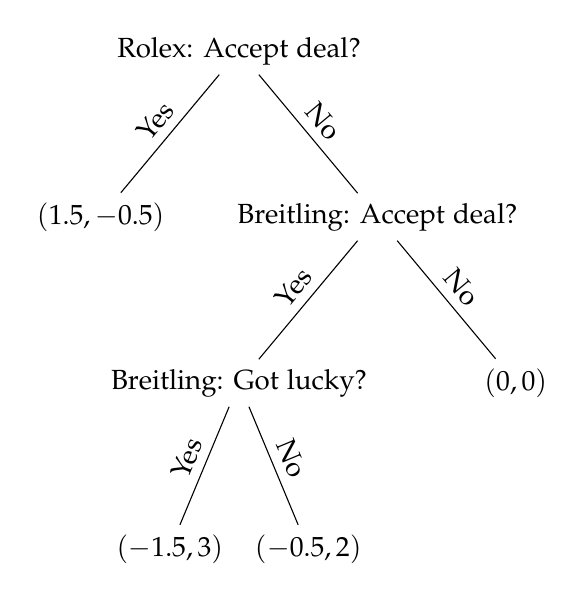
\begin{tikzpicture}[
  level distance = 6em,
  level 1/.style = {sibling distance = 10em},
  level 2/.style = {sibling distance = 10em},
  level 3/.style = {sibling distance = 5em},
  sloped
]

\node {Rolex: Accept deal?}
  child {
    node {$(1.5,-0.5)$}
    edge from parent node [above] {Yes}
  }
  child {
    node {Breitling: Accept deal?}
      child {
        node {Breitling: Got lucky?}
          child {
            node {$(-1.5,3)$}
            edge from parent node [above] {Yes}
          }
          child {
            node {$(-0.5,2)$}
            edge from parent node [above] {No}
          }
        edge from parent node [above] {Yes}
      }
      child {
        node {$(0,0)$}
        edge from parent node [above] {No}
      }
    edge from parent node [above] {No}
  };

\end{tikzpicture}
\end{center}

This game has an element of uncertainty. When Breitling accepts the deal,
this company can get lucky. But we don't know for sure if that's going to
happen. We only know the corresponding probability: \(p=0.5\). To be
honest, I'm not sure about how to deal with this kind of game. Perhaps I'm
wrong, but I believe the lectures don't cover this topic. So I'll adopt the
approach that seems most reasonable to me. Specifically, I'm going to
replace the sub-tree rooted at ``Breitling: Got lucky?'' with a leaf node.
This node will contain the expectation values of the payoffs for Rolex and
Breitling. For Rolex, this expectation value can be computed as follows:
\begin{align*}
E[p_R]&=(-1.5)p+(-0.5)(1-p)\\
&=-1.5p-0.5(1-p)\\
&=-1.5p-0.5+0.5p\\
&=-p-0.5\\
&=-0.5-0.5\\
&=-1.
\end{align*}
Similarly, for Breitling we can write the following:
\begin{align*}
E[p_B]&=3p+2(1-p)\\
&=3p+2-2p\\
&=p+2\\
&=0.5+2\\
&=2.5.
\end{align*}
By using these results, we can draw the new game tree:
\begin{center}
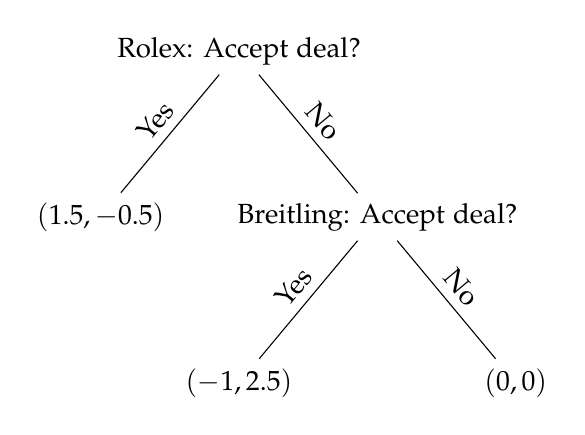
\begin{tikzpicture}[
  level distance = 6em,
  level 1/.style = {sibling distance = 10em},
  level 2/.style = {sibling distance = 10em},
  sloped
]

\node {Rolex: Accept deal?}
  child {
    node {$(1.5,-0.5)$}
    edge from parent node [above] {Yes}
  }
  child {
    node {Breitling: Accept deal?}
      child {
        node {$(-1,2.5)$}
        edge from parent node [above] {Yes}
      }
      child {
        node {$(0,0)$}
        edge from parent node [above] {No}
      }
    edge from parent node [above] {No}
  };

\end{tikzpicture}
\end{center}

Next, we apply backward induction to determine the outcome of this game. We
begin by analyzing the sub-tree rooted at ``Breitling: Accept deal?''. From
Breitling's perspective, the choice is between making no additional profit
or increasing its profit by \pounds2.5 million. Then, if this company has
the chance, it should accept the deal.\\
Finally, consider what Rolex should do. If this company does \textbf{not} accept
the deal, then its competitor will. In this case, Rolex loses money: its
gross profit decreases by \pounds1 million. On the other hand, if this firm
accepts the deal, it will earn an additional profit of \pounds1.5 million.
This makes it clear that, for Rolex, the best option is to accept the deal.
As the CEO of this company, that's exactly what I would do.
\section*{Problem 19}
\label{sec:org3fae9a1}

\textbf{Answer:} False\\

This question is very similar to the first question of Quiz 1. In the
solution to that quiz, we concluded that a Nash equilibrium with dominated
strategies cannot exist.
\section*{Problem 20}
\label{sec:org21abd82}

\textbf{Answer:}
\begin{itemize}
\item Limit pricing means that firms are bound to a price cap introduced by the
competition authority.
\end{itemize}
\section*{Problem 21}
\label{sec:org9fd7da9}

\textbf{Answer:}
\begin{itemize}
\item Perfect market transparency
\item No capacity constraints
\item Infinite price elasticity
\item Identical products
\end{itemize}
\section*{Problem 22}
\label{sec:org2d060c2}

\textbf{Answer:} False
\section*{Problem 23}
\label{sec:orgebca2b8}

\textbf{Answer:} False
\section*{Problem 24}
\label{sec:org71efbc8}

\textbf{Answer:} \ldots{}it affects the elasticity of demand of the focal product.
\section*{Problem 25}
\label{sec:orga8119b1}

\textbf{Answer:} Pizza Hut - Medium Price / Domino's Pizza - Medium Price\\

First, consider the best reply by Pizza Hut for each strategy of Domino's
Pizza:
\begin{itemize}
\item Domino's Pizza charges a High price: Pizza Hut charges a High price;
\item Domino's Pizza charges a Medium price: Pizza Hut charges a Medium price;
\item Domino's Pizza charges a Low price: Pizza Hut charges a Medium price.
\end{itemize}
Next, consider the best reply by Domino's Pizza for each strategy of Pizza
Hut:
\begin{itemize}
\item Pizza Hut charges a High price: Domino's Pizza charges a Medium price;
\item Pizza Hut charges a Medium price: Domino's Pizza charges a Medium price;
\item Pizza Hut charges a Low price: Domino's Pizza charges a Low price.
\end{itemize}
This makes it clear that this game has a Nash equilibrium characterized by
both companies charging a medium price. Since the two players are rational,
the outcome of this game corresponds to this Nash equilibrium.
\end{document}
